\begin{abstract}
High-dimensional hidden-state streams offer a data source for mining the evolving safety risk of large language model responses. We develop a reproducible workflow integrating data cleaning, dimensionality reduction, feature engineering, sequence classification and cluster analysis. Frozen Qwen2.5 states are compressed by train-only incremental principal component analysis (PCA); state differences and geometric changes describe prefix evolution. Term frequency--inverse document frequency (TF--IDF) and linear probes provide text and representation baselines, while a gated recurrent unit (GRU) models the feature sequence. Independent sequence-level calibration converts scores into streaming decisions, and K-means profiles the structure of response representations. \ReviewRankingEN{} \AbstractResultsEN{} Static and temporal detectors provide distinct recall--false-positive-rate profiles. Shared feature caches and a buffer-check-release interface connect offline data mining with incremental operation, providing an accessible experimental framework for resource-conscious content-safety analysis.
\end{abstract}
\begin{IEEEkeywords}
data mining, principal component analysis, feature engineering, clustering, sequence classification, hidden states, large language models, streaming safety detection
\end{IEEEkeywords}

\section{Introduction}
Large language models deliver responses token by token, whereas many safety datasets assign a judgment to the complete answer. This creates a practical learning problem: how can a monitor use the currently visible prefix to identify responses that will ultimately be labelled unsafe, while keeping whole-response false alarms and monitoring cost under control? For example, the same prompt may receive a safe explanation or an unsafe continuation; reading the evolving response adds evidence beyond the question alone.

From a data-mining perspective, each answer is a variable-length multivariate sequence, each checkpoint is a high-dimensional observation, and the final safety judgment is its supervised label. Data cleaning and grouped partitioning establish the analysis population; PCA compresses the observations; temporal feature engineering and classification estimate risk; unsupervised clustering describes recurring representation profiles. These stages organize the study as a complete data-to-pattern-to-decision workflow.

Three design requirements follow. The representation must respect the visible-prefix boundary; the detector must distinguish useful contextual information from the additional value of temporal modeling; and the decision rule must account for repeated checks throughout a response. Under local resource constraints, these requirements also call for compact features and reusable extraction artifacts.

SCM combines fine-grained supervision with hierarchical consistency-aware training~\cite{NEURIPS2025_4e315702}, while Kelp learns temporal risk heads from frozen representations~\cite{li2025kelpstreamingsafeguardlarge}. Building on this foundation, we address the requirements through a common experimental pipeline: causal replay supplies aligned hidden states, train-only projection compresses multi-layer features, matched detector families compare static and temporal information, and independent sequence-level calibration converts scores into streaming decisions. A buffer-check-release interface carries the same features into incremental generation.

The investigation follows three questions. RQ1: what predictive information do hidden states and temporal modeling contribute relative to prompt and prefix-text baselines? RQ2: how does checkpoint frequency change detection coverage and monitoring work? RQ3: how do backbone scale and response source affect the resulting operating profiles? Each question is linked to a controlled comparison and a corresponding results subsection.

The contributions are a reproducible causal representation-mining workflow, measured evidence for detector and checkpoint selection, and an incremental monitoring implementation with traceable artifacts. \AchievementScopeEN{} The evidence establishes compact hidden states as useful risk-ranking features and quantifies the recall--FPR choices offered by static and recurrent heads. Sections~\ref{sec:architecture} and~\ref{sec:protocol} describe the solution; Section~\ref{sec:results} answers the research questions.

\section{Related Work}
\subsection{Safety Annotation and Response Moderation}
BeaverTails provides question--answer safety annotations and distinguishes helpfulness from harmlessness~\cite{ji2023beavertails}. Its response-level labels support the eventual-outcome prediction task studied here. We retain the original response judgment and category metadata, with prompt intent and response safety represented as distinct variables.

WildGuard jointly studies prompt intent, response safety and refusal detection~\cite{han2024wildguard}. These complementary targets motivate the prompt-only control and the comparison between prompt information and observed response features.

FineHarm supplies sentence labels and uses a part-of-speech heuristic to derive word labels aligned to tokens~\cite{NEURIPS2025_4e315702}. This fine-grained annotation route complements the complete-response supervision used in the present study.

\subsection{Streaming Monitoring from Internal Representations}
SCM trains a separate Qwen2.5-based monitor with token and holistic response heads, retaining the token head at inference~\cite{NEURIPS2025_4e315702}. Kelp attaches a lightweight temporal head to a frozen target model and introduces anchored temporal consistency for response-level supervision~\cite{li2025kelpstreamingsafeguardlarge}. These designs connect representation access, supervision granularity and sequential decision making.

Our detector family combines projected states, causal state differences and a standard unidirectional GRU~\cite{cho2014gru}. The response-level objective and modular feature construction support direct comparisons of current state, accumulated history and learned temporal aggregation.

StreamGuard constructs future-risk targets using Monte Carlo continuations~\cite{kavumba2026streamguard}, while online risk-control monitoring calibrates an external verifier signal~\cite{schirmer2026online}. SafeDecoding intervenes through token-probability adjustment during generation~\cite{xu2024safedecoding}. Together, these approaches situate the present work within a broader design space of risk prediction, decision calibration and generation control.

Recent work also explores token-level hidden-state probes~\cite{shu2026stopearly}, pretrained sparse-autoencoder features~\cite{fang2026nextguard} and adaptive depth--time monitoring~\cite{wei2026adtguard}. These approaches extend the representation and supervision design space. The present study focuses on a reproducible small-backbone comparison using shared response partitions and sequence-level calibration.

\subsection{Replay, Native Generation and Transfer}
StreamGuardBench supplies responses generated by specific target models~\cite{li2025kelpstreamingsafeguardlarge,streamguardbench2025data}. Replaying these responses through a fixed monitoring backbone supports representation comparisons across response sources. We record the response-generating source and the monitoring encoder separately.

External evaluation keeps the fitted detector and its threshold fixed while changing the response source, prompting distribution and annotation process. This design measures transport of the complete monitoring pipeline across data sources.

\section{Task Definition and Evaluation Contract}
\subsection{Observed Prefix and Prediction Target}
Let $q_i$ be a prompt and $r_i=(r_{i,1},\ldots,r_{i,T_i})$ an annotated response. The binary label $Y_i$ indicates whether the complete response is unsafe. At response checkpoint $t\leq T_i$, a detector receives only the prompt and the first $t$ response tokens and returns
\begin{equation}
 \risk_{i,t}=f_\theta(q_i,r_{i,1:t}).
 \label{eq:target}
\end{equation}
Equation~\ref{eq:target} defines a ranking score for the final response label $Y_i=1$, conditional on the observed prefix. Class-weighted training emphasizes the prediction target, and the operational threshold is determined by the separate calibration stage.

Checkpoints form an ordered set $\mathcal T_i$. The full endpoint $T_i$ is always included. For threshold $\tau$, the alarm location and sequence decision are
\begin{align*}
 A_i(\tau)&=\min\{t\in\mathcal T_i:\risk_{i,t}>\tau\},\\
 D_i(\tau)&=\mathbb{1}\{\max_{t\in\mathcal T_i}\risk_{i,t}>\tau\},
\end{align*}
Here $A_i=\infty$ denotes an untriggered response. The strict $>$ comparison is saved with the threshold and reused throughout calibration, replay and online inference.

\subsection{Primary Endpoint}
For observed-token budget $B$, early recall is
\begin{equation}
 R_B=\frac{\sum_i\mathbb{1}\{Y_i=1,\ A_i\leq\min(B,T_i)\}}
 {\sum_i\mathbb{1}\{Y_i=1\}}.
 \label{eq:recall}
\end{equation}
The primary endpoint is $R_{128}$, with secondary budgets of 32, 64 and 256 tokens. A budget includes all checkpoints observed up to $\min(B,T_i)$; shorter responses contribute their true endpoint. Supplementary timing analysis additionally requires the alarm checkpoint to precede the response endpoint.

Sequence-level false-positive rate (FPR) is the proportion of safe complete responses for which $D_i=1$. We also report precision, recall and F1 from sequence decisions and ranking measures from the maximum response score. An apparently small per-checkpoint error can accumulate across many checkpoints, so threshold calibration and false-positive reporting both operate at the sequence level.

Alarm-location summaries describe detected unsafe responses and are reported alongside recall. The normalized location $A_i/T_i$ provides a response-relative timing measure during evaluation; complete response length is used only to calculate this metric.

\section{Architecture and Data Flow}\label{sec:architecture}
\begin{figure*}[t]
\centering
\IfFileExists{figures/architecture.pdf}{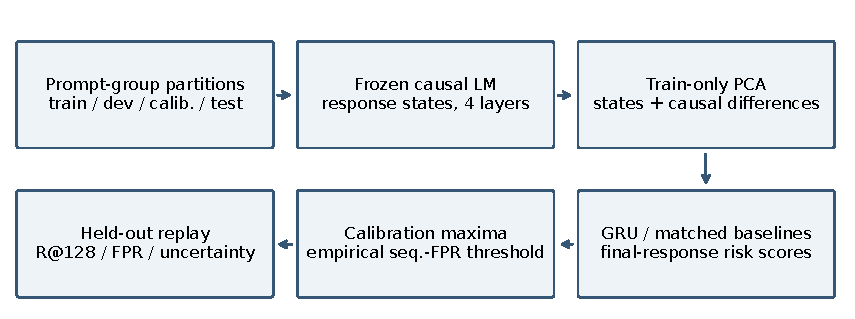
\includegraphics[width=.98\textwidth]{figures/architecture.pdf}}{\fbox{Architecture diagram pending report generation.}}
\caption{Experimental data flow. Detector features are fitted only on training records; test labels do not select models or thresholds. Test text is used only for the disclosed overlap audit during corpus construction. The schematic connects the experiment stages and their artifacts.}
\label{fig:architecture}
\end{figure*}

The architecture implements three linked steps. First, grouped data preparation and causal extraction define what information is available at each checkpoint. Second, projection and matched detector families test how that information should be represented and aggregated. Third, sequence-level calibration and buffered release translate scores into operational decisions. This progression connects the prediction problem to both the comparative experiments and the online interface.

\subsection{Data Cleaning and Grouped Partitioning}
The primary source is the BeaverTails 30k training partition. The configured target allocation is 8,000 training responses, 1,000 development responses and 1,000 calibration responses, subject to eligibility and prompt-group constraints. The official test partition supplies all retained eligible test responses. These are design allocations; observed retained counts are generated from the processed files in Table~\ref{tab:dataset}.

Records store an identifier, normalized prompt group, split, source, response label, available categories, text, token identifiers and response length. Normalized prompt groups prevent multiple answers to the same normalized question from crossing partitions. The official tests receive priority: matching prompts and response templates are removed from the candidate training pool. Character TF--IDF nearest-neighbor comparison also removes candidate prompt groups close to test prompts at similarity 0.92. This text-only audit transform is not reused by the detector and reads no test labels. Exact response templates are additionally isolated across training, development and calibration. Retained identifiers and source revisions make these decisions inspectable independently of training.

The configured tokenizer applies eligibility limits of 256 prompt tokens and 512 response tokens. Eligible responses retain their complete text and original labels. The audit records length exclusions, invalid records, class counts and retained sample identifiers.

The external source is the original StreamGuardBench \texttt{wildguard\_qwen3\_8b} test partition, identified by an immutable dataset revision~\cite{streamguardbench2025data}. Preparation retains the original response label and uses prompt and response text as predictor inputs. Duplicate conflicts give priority to held-out tests, and all source revisions, exclusions and retained records are preserved in the audit.

\begin{table}[t]
\centering\footnotesize
\caption{Observed retained responses after length filtering, grouping and deduplication.}\label{tab:dataset}
\begin{tabular}{lrrr}\toprule
Split & $N$ & Unsafe & Groups \\
\midrule
calibration & 1001 & 563 & 275 \\
dev & 1003 & 551 & 282 \\
external & 591 & 54 & 591 \\
test & 3018 & 1732 & 2524 \\
train & 7997 & 4560 & 2211 \\
\bottomrule\end{tabular}
\end{table}

The eligibility audit retains 591 of 1,725 external responses (34.3\%), including 54 of 284 originally unsafe responses. The retained external unsafe prevalence is 9.1\%. Exclusion reasons and class-specific retention are preserved in the audit and source data.

\resultfigure{data_class_balance}{Class composition of retained responses. Counts refer to responses; prompt-group counts are reported separately in Table~\ref{tab:dataset}. Bars show the retained response counts by final label.}{Dataset composition awaits processed records.}
\resultfigure{external_retention}{Class-specific retention of the external test source after eligibility filtering. Labels give retained/original counts. Differential retention changes the evaluation population.}{External eligibility audit is pending.}

\subsection{Frozen Causal Feature Extraction}
The feature backbone is Qwen2.5-0.5B-Instruct~\cite{qwen2024qwen25}. Its weights remain frozen, and FP16 extraction reduces the activation footprint. We sample returned hidden-state indices 6, 12, 18 and 24; the final index includes the backbone's terminal RMSNorm. Prompt formatting and tokenizer identity are fixed across partitions. Extraction uses the causal attention structure: the representation of a response position depends only on its prompt and preceding visible response context.

Teacher-forced replay computes monitoring representations of each recorded answer under causal attention. For the external Qwen3-8B responses, the encoder is the frozen Qwen2.5 monitoring model. This setup separates representation extraction from the response source and enables controlled detector comparisons.

Raw features are cached at a base stride of four response tokens, with the final token appended if needed. The principal detector uses stride eight; stride-four and stride-sixteen variants reuse the same cache. This design separates expensive backbone extraction from the relatively inexpensive detector comparisons. Cache metadata records layer order, token positions and preprocessing identity to prevent a detector from silently consuming a different representation.

\subsection{Incremental PCA and Temporal Feature Engineering}
For layer $\ell$, let $h^{(\ell)}_{i,t}\in\mathbb R^d$ be a causal hidden state. Incremental principal component analysis (PCA) fits a 64-dimensional projection using training responses only. PCA summarizes covariance structure along orthogonal high-variance directions~\cite{jolliffe2016pca}; fitting it in batches supports memory-conscious processing of checkpoint observations. Its role here is unsupervised feature compression before supervised classification. At most eight checkpoints are sampled from each training answer, capping the contribution of long responses. A residual fitting batch with fewer than 64 rows is omitted and counted in metadata; these responses remain available for transformation and detector training. Each layer is transformed separately:
\begin{equation*}
 z^{(\ell)}_{i,t}=\operatorname{diag}(\max(\lambda_\ell,\epsilon))^{-1/2}
 P_\ell(h^{(\ell)}_{i,t}-\mu_\ell).
\end{equation*}
Here $\lambda_\ell$ contains the training explained variances; division by their square roots whitens the projected states, with a numerical floor $\epsilon=10^{-8}$. The fitted means, projections and variances are reused unchanged for development, calibration and both tests. This is an inductive experiment; fitting PCA on the combined dataset would introduce a transductive dependency even without labels.

\PCAVarianceEN{}

At each selected layer, we concatenate the whitened state $z_t$, difference $z_t-z_{t^-}$, cosine change $1-\cos(z_t,z_{t^-})$, and norm change $\|z_t\|_2-\|z_{t^-}\|_2$. The four-layer input has $4(64+64+1+1)=520$ dimensions; the last-layer ablation has 130. All change features are zero at the first checkpoint. When stride changes, differences are recomputed between the actually selected checkpoints rather than subsampled from a different stride. Feature scaling is also fit only on training checkpoints with response-balanced sample weights. This keeps every data-dependent transformation upstream of validation and threshold selection.

\subsection{Detectors and Matched Baselines}
The main temporal model is a single-layer unidirectional GRU with hidden size 64 and a linear scalar output. For feature vector $x_{i,t}$ and recurrent state $s_{i,t}$,
\begin{equation*}
 s_{i,t}=\operatorname{GRU}(x_{i,t},s_{i,t^-}),\quad
 \risk_{i,t}=\sigma(w^\top s_{i,t}+b),
\end{equation*}
where $t^-$ is the preceding checkpoint. The hidden state resets at every response boundary. Right padding is excluded from supervision and evaluation; it cannot affect earlier valid outputs of the unidirectional network.

Four baselines test specific alternative explanations. Prompt-only logistic regression measures how much risk is predictable before reading the response. Prefix TF--IDF logistic regression uses the prompt and currently visible response text with train-only word and character vocabularies. Current-state logistic regression tests whether the present projected representation is sufficient. Running-mean logistic regression tests causal history aggregation without learned recurrence. These models use the same final-response target and evaluation rule.

The text representation concatenates word 1--2-grams and within-word character 3--5-grams, each capped at 20,000 features, with sublinear term frequency. Linear models use $C=1$, response-balanced class weights and the liblinear solver with a 500-iteration cap.

Ablations remove state-change features, retain the final selected layer, replace recurrent aggregation with a current-checkpoint MLP, or use checkpoint strides of four and sixteen tokens. These variants characterize feature construction and aggregation choices under the common data and calibration protocol.

\subsection{Incremental Monitoring Contract}
The online interface consumes each token before computing its checkpoint state. It buffers the current token block, releases it after a non-alert decision, and discards the block and stops generation after an alert. A final partial block is checked at EOS, and every response resets detector and feature-builder state.

\section{Training, Calibration and Uncertainty}\label{sec:protocol}
\subsection{Response-Balanced Weak Prefix Supervision}
Up to eight evenly spaced checkpoints per training response, including its endpoint, contribute supervised loss. If $\mathcal S_i$ is this selected set, the neural objective is
\begin{equation}
 \mathcal L=\frac{1}{N}\sum_{i=1}^N\frac{1}{|\mathcal S_i|}
 \sum_{t\in\mathcal S_i}\operatorname{BCE}_{w_+}(a_{i,t},Y_i),
 \label{eq:loss}
\end{equation}
where $a$ denotes the pre-sigmoid logit and $w_+=N_0/N_1$ weights positive responses. The inner average prevents long answers from receiving more loss weight merely because they contain more checkpoints. Linear models likewise use inverse-prefix-count sample weights and response-count class weights.

Equation~\ref{eq:loss} implements response-balanced weak prefix supervision. Each checkpoint predicts the same eventual outcome, while prompt-only controls and feature ablations characterize the contribution of the available information. The objective trains scores across the observed sequence using the shared response target.

Neural models use AdamW with configured learning rate $10^{-3}$ and weight decay $10^{-4}$, batch size 32, gradient clipping at 1.0 and at most 20 epochs. Development maximum-score ROC AUC selects checkpoints, with patience three. The seeds 13, 42 and 2026 are specified in advance. The development set selects model states; the distinct calibration set selects operational thresholds. Test measurements do not select either.

\subsection{Empirical Sequence-Level Calibration}
For each safe calibration response, define $M_i=\max_t\risk_{i,t}$. Sort its $n_0$ values as $M_{(1)}\leq\cdots\leq M_{(n_0)}$. With target $\alpha=0.05$ and $k=\lfloor\alpha n_0\rfloor$, the implemented threshold is
\begin{equation*}
 \tau=M_{(n_0-k)}.
\end{equation*}
Under the strict $>$ alarm rule, at most $k$ safe calibration responses cross the threshold; tied values can produce a smaller empirical rate. Test performance is reported through the resulting recall and measured sequence-level FPR.

Each method and seed receives a threshold from the same calibration procedure and target, accommodating differences in score scale. External evaluation carries forward the fitted detector and its in-domain threshold.

\subsection{Grouped Paired Estimation}
Point estimates are summarized by the mean and sample standard deviation across fixed seeds. Prompt groups define the resampling unit, preserving the relationship between answers to the same question during uncertainty estimation.

The paired bootstrap draws prompt groups with replacement 1,000 times and retains all answers in each selected group. Each draw is shared across the compared methods and their common seeds, with scores and thresholds fixed. Contrasts are challenger minus reference, and 95\% percentile intervals use the 2.5th and 97.5th percentiles.

Recall@128 defines the primary contrast. Secondary metrics, ablations and exploratory sensitivity analyses are identified in their tables and archived with the complete per-seed measurements.

\section{Experimental Results}\label{sec:results}
The results answer the three research questions in order, followed by system measurements and exploratory representation analysis. Recall is interpreted jointly with measured test FPR under the common 5\% calibration target.
\subsection{RQ1: Representation and Detector Selection}
\paragraph{Complete-pipeline comparison.}\AchievementDetectionEN{} Paired prompt-group uncertainty is reported in Table~\ref{tab:uncertainty}.

\begin{table}[t]
\centering\footnotesize
\caption{In-domain detection (\%). Mean $\pm$ sample SD across available seeds; a single completed seed has no SD. Thresholds use only in-domain calibration.}\label{tab:main}
\begin{tabular}{lrrrr}\toprule
Method & R@128 & FPR & AUROC & AP \\
\midrule
Prompt LR & 22.9 $\pm$ 0.0 & 3.3 $\pm$ 0.0 & 74.4 $\pm$ 0.0 & 80.1 $\pm$ 0.0 \\
Prefix TF--IDF LR & 28.2 $\pm$ 0.0 & 1.6 $\pm$ 0.0 & 81.1 $\pm$ 0.0 & 86.3 $\pm$ 0.0 \\
Current-state LR & 43.7 $\pm$ 0.0 & 5.6 $\pm$ 0.0 & 83.1 $\pm$ 0.0 & 86.5 $\pm$ 0.0 \\
Running-mean LR & 46.1 $\pm$ 0.0 & 6.2 $\pm$ 0.0 & 83.5 $\pm$ 0.0 & 86.5 $\pm$ 0.0 \\
Dynamic GRU & 38.1 $\pm$ 6.3 & 3.3 $\pm$ 1.0 & 83.6 $\pm$ 0.9 & 87.6 $\pm$ 0.8 \\
\bottomrule\end{tabular}
\end{table}


\paragraph{Detector trade-offs.}Table~\ref{tab:main} reports the full baseline comparison. Static probes, MLPs and recurrent heads offer complementary recall--FPR profiles under the common calibration target, supporting application-specific detector selection.

\begin{table}[t]
\centering\footnotesize
\caption{In-domain alert positions. Timing is conditional on true detections; recall retains all unsafe responses in its denominator.}\label{tab:alert_positions}
\begin{tabular}{lrrrr}\toprule
Method & Recall & Mean $\tau$ & Med. $\tau$ & $\tau/T$ (\%) \\
\midrule
Prompt LR & 22.9 $\pm$ 0.0 & 8.0 $\pm$ 0.0 & 8.0 $\pm$ 0.0 & 14.8 $\pm$ 0.0 \\
Prefix TF--IDF LR & 28.3 $\pm$ 0.0 & 20.7 $\pm$ 0.0 & 8.0 $\pm$ 0.0 & 26.2 $\pm$ 0.0 \\
Current-state LR & 43.9 $\pm$ 0.0 & 27.5 $\pm$ 0.0 & 16.0 $\pm$ 0.0 & 34.6 $\pm$ 0.0 \\
Running-mean LR & 46.3 $\pm$ 0.0 & 15.1 $\pm$ 0.0 & 8.0 $\pm$ 0.0 & 23.5 $\pm$ 0.0 \\
Dynamic GRU & 38.4 $\pm$ 6.1 & 47.9 $\pm$ 15.1 & 41.8 $\pm$ 18.3 & 54.0 $\pm$ 11.5 \\
\bottomrule\end{tabular}
\end{table}


\begin{table}[t]
\centering\footnotesize
\caption{Prompt-group paired bootstrap: Recall@128 differences and 95\% intervals (percentage points).}\label{tab:uncertainty}
\begin{tabular}{lp{.34\columnwidth}rr}\toprule
Split & Contrast & $\Delta$ & 95\% CI \\
\midrule
test & Dynamic GRU vs. Prompt LR & +15.2 & [+12.7, +17.8] \\
test & Dynamic GRU vs. Current-state LR & -5.6 & [-7.1, -3.9] \\
test & Dynamic GRU vs. Prefix TF--IDF LR & +9.9 & [+7.6, +12.2] \\
external & Dynamic GRU vs. Prompt LR & +12.3 & [+6.7, +18.8] \\
external & Dynamic GRU vs. Current-state LR & -11.7 & [-20.6, -3.6] \\
external & Dynamic GRU vs. Prefix TF--IDF LR & +12.3 & [+6.7, +18.8] \\
\bottomrule\end{tabular}
\end{table}


\paragraph{Same-prompt outcomes.}The test subset containing both final labels per prompt has 97 groups and 207 responses. Dynamic GRU and current-state LR attain 20.1\% and 22.3\% Recall@128, at 6.1\% and 6.7\% FPR, respectively, using unchanged thresholds. The matched-prompt subset characterizes how the two detectors respond to different outcomes associated with a shared question.

\paragraph{History-aggregation control.}Running-mean LR obtains 46.1\% Recall@128; the dynamic-GRU difference is -8.1 percentage points. The comparison complements current-state and learned-recurrence baselines by quantifying causal history accumulation.

\paragraph{Uncertainty.}Table~\ref{tab:uncertainty} retains paired prompt-group bootstrap intervals. Each paired draw preserves the prompt groups and fixed fitted seeds across the compared detectors.

\paragraph{Pre-specified contrast.}The dynamic-GRU minus static-probe Recall@128 difference is -5.64 percentage points (95\% prompt-group interval [-7.10, -3.93]). The static probe favors recall coverage, while the GRU has the lower observed test FPR; these operating profiles support different monitoring priorities.

\paragraph{Supplementary ranking and calibration.}

\ReviewRankingEN{} AUROC@128 uses the maximum score within the token budget, with intervals from 1,000 paired prompt-group bootstrap draws. The within-family linear comparison provides complementary evidence about the two feature constructions.

The GRU and static probe have similar budgeted ranking estimates: the AUROC@128 difference is 0.0050, with a 95\% interval of [-0.0019, 0.0123].

Table~\ref{tab:review_sensitivity} compares operating profiles at calibration targets of 1\%, 5\% and 10\%, holding the fitted models fixed and retaining 5\% as the primary setting.\begin{table}[t]
\centering\footnotesize
\caption{Post-hoc exploratory calibration-target analysis: means over three fixed seeds (\%). Calibration data select thresholds; 5\% is primary. Comparison intervals are unadjusted.}\label{tab:review_sensitivity}
\begin{tabular}{lrrr}\toprule
Method & $\alpha$ & R@128 & Test FPR \\
\midrule
Prefix TF--IDF LR & 1 & 12.9 & 0.3 \\
Current-state LR & 1 & 18.0 & 1.2 \\
Dynamic GRU & 1 & 18.5 & 1.0 \\
Prefix TF--IDF LR & 5 & 28.2 & 1.6 \\
Current-state LR & 5 & 43.7 & 5.6 \\
Dynamic GRU & 5 & 38.1 & 3.3 \\
Prefix TF--IDF LR & 10 & 43.7 & 5.5 \\
Current-state LR & 10 & 61.7 & 13.5 \\
Dynamic GRU & 10 & 56.2 & 9.0 \\
\bottomrule\end{tabular}
\end{table}


The strict pre-completion criterion requires an alarm checkpoint before the answer endpoint and within 128 tokens. With all unsafe responses retained in the denominator, main-test recall is 42.8\% for the static probe and 35.1\% for GRU. This timing view complements the budgeted recall curves.


\resultfigure{recall_budget_test}{Unsafe-response recall at visible-token budgets on the in-domain test split. Points and error bars show means and one sample SD across completed seeds; a single seed has no SD. Thresholds remain frozen.}{No completed recall curves are available.}

\subsection{RQ2: Checkpoint Frequency and Feature Ablations}
Table~\ref{tab:ablation} and the ablation figure compare feature, aggregation and stride choices. States-only GRU retains recurrence while removing changes; the dynamic MLP retains the input features while replacing memory. The stride comparison changes the next permitted alarm and the number of scoring operations, with dynamic features recomputed at each stride. These comparisons identify practical design choices within the same extraction and calibration pipeline.
\StrideResultsEN{}
\begin{table}[t]
\centering\footnotesize
\caption{Ablation and checkpoint-stride sensitivity (\%).}\label{tab:ablation}
\begin{tabular}{lrr}\toprule
Setting & R@128 & Seq. FPR \\
\midrule
Dynamic GRU & 38.1 $\pm$ 6.3 & 3.3 $\pm$ 1.0 \\
GRU, states only & 41.2 $\pm$ 3.2 & 3.3 $\pm$ 0.8 \\
GRU, last layer & 33.3 $\pm$ 0.9 & 2.7 $\pm$ 0.2 \\
Dynamic MLP & 47.7 $\pm$ 4.1 & 5.1 $\pm$ 1.2 \\
GRU, stride 4 & 40.5 $\pm$ 4.2 & 3.0 $\pm$ 0.9 \\
GRU, stride 16 & 37.0 $\pm$ 2.2 & 3.5 $\pm$ 0.2 \\
\bottomrule\end{tabular}
\end{table}

\resultfigure{ablations}{Measured Recall@128 for temporal, feature and checkpoint-stride comparisons. Bars and errors show means and one sample SD across completed seeds, respectively. Each setting uses the common response partitions and calibration procedure.}{Ablation measurements are pending.}

\subsection{RQ3: Backbone Scale and Response-Source Transfer}
The scale experiment changes the monitoring backbone while keeping response partitions fixed. The external experiment changes the response source while carrying forward the fitted detector and threshold. Together, they distinguish representation scaling from transport of the complete decision rule.
\AchievementScaleEN{}
\paragraph{Backbone scale.}Table~\ref{tab:scale} compares frozen 0.5B and 1.5B representations on identical response partitions. The 1.5B model uses returned hidden-state indices 7, 14, 21 and 28, with the same per-layer projection dimension and training protocol. Both configurations encode the same response partitions.\begin{table}[t]
\centering\footnotesize
\caption{Backbone-scale validation on identical responses (\%); each size has independently fitted transformations, probes and calibration thresholds.}\label{tab:scale}
\begin{tabular}{llrrr}\toprule
Size & Method & R@128 & FPR & Ext. R@128 \\
\midrule
0.5B & Current-state LR & 43.7 $\pm$ 0.0 & 5.6 $\pm$ 0.0 & 24.1 $\pm$ 0.0 \\
0.5B & Dynamic GRU & 38.1 $\pm$ 6.3 & 3.3 $\pm$ 1.0 & 12.3 $\pm$ 13.4 \\
1.5B & Current-state LR & 54.0 $\pm$ 0.0 & 5.8 $\pm$ 0.0 & 25.9 $\pm$ 0.0 \\
1.5B & Dynamic GRU & 49.6 $\pm$ 4.6 & 4.9 $\pm$ 1.7 & 17.3 $\pm$ 2.8 \\
\bottomrule\end{tabular}
\end{table}


\begin{table}[t]
\centering\footnotesize
\caption{External detection (\%). Mean $\pm$ sample SD across available seeds; a single completed seed has no SD. Thresholds use only in-domain calibration.}\label{tab:external}
\begin{tabular}{lrrrr}\toprule
Method & R@128 & FPR & AUROC & AP \\
\midrule
Prompt LR & 0.0 $\pm$ 0.0 & 4.7 $\pm$ 0.0 & 48.2 $\pm$ 0.0 & 8.2 $\pm$ 0.0 \\
Prefix TF--IDF LR & 0.0 $\pm$ 0.0 & 1.3 $\pm$ 0.0 & 62.0 $\pm$ 0.0 & 12.8 $\pm$ 0.0 \\
Current-state LR & 24.1 $\pm$ 0.0 & 8.6 $\pm$ 0.0 & 80.0 $\pm$ 0.0 & 31.0 $\pm$ 0.0 \\
Running-mean LR & 11.1 $\pm$ 0.0 & 2.6 $\pm$ 0.0 & 80.8 $\pm$ 0.0 & 27.8 $\pm$ 0.0 \\
Dynamic GRU & 12.3 $\pm$ 13.4 & 5.0 $\pm$ 1.1 & 81.0 $\pm$ 1.9 & 33.1 $\pm$ 4.4 \\
\bottomrule\end{tabular}
\end{table}


\paragraph{Transfer boundary.}The external results use the frozen in-domain threshold. They therefore test transport of the complete scoring-and-threshold rule. Differences in source models, annotation policies and response lengths can each contribute to a transfer gap.
External GRU detections within 128 tokens are 2, 15, 3 out of 54 unsafe responses for seeds 13, 42 and 2026. Seed 42 gives 15/54, with a descriptive Wilson 95\% interval of [17.6, 40.9]\%. The archive provides per-seed counts and intervals for both recall and FPR.

\resultfigure{recall_budget_external}{External early recall with unchanged in-domain thresholds. Error bars show one seed SD, as in the in-domain plot. This is response-source transfer under replay.}{External measurements are pending.}

\subsection{System Feasibility and Incremental Operation}
System measurements connect the detection study to local execution: shared caches amortize backbone extraction, checkpoint timings quantify added monitoring work, and incremental replay checks score consistency between offline and KV-based operation.
\begin{table}[t]
\centering\footnotesize
\caption{Measured fit time and detector-only latency, averaged across seeds. Head timing excludes backbone, tokenization, PCA and dynamic-feature construction.}\label{tab:timing}
\begin{tabular}{lrrr}\toprule
Method & Fit (s) & p50 (ms) & p95 (ms) \\
\midrule
Prompt LR & 5.44 & -- & -- \\
Prefix TF--IDF LR & 29.34 & -- & -- \\
Current-state LR & 5.67 & -- & -- \\
Running-mean LR & 5.37 & -- & -- \\
Dynamic GRU & 36.20 & 0.21 & 0.26 \\
GRU, states only & 34.16 & 0.21 & 0.26 \\
GRU, last layer & 42.33 & 0.20 & 0.28 \\
Dynamic MLP & 31.21 & 0.14 & 0.16 \\
GRU, stride 4 & 47.50 & 0.21 & 0.27 \\
GRU, stride 16 & 24.60 & 0.21 & 0.30 \\
\bottomrule\end{tabular}
\end{table}

\paragraph{Matched-length generation.}Across 3 warmed paired trials on the fixed benign demonstration prompt, median baseline and monitor-only generation times are 2.267 and 2.250 s, respectively. The median paired overhead is -0.1\%. Each pair has an identical greedy token-sequence hash; model-loading time is excluded. The paired design profiles checkpoint monitoring within the same generation workload.

The observed paired ratios range from -5.4\% to +6.2\%. The paired measurements place monitored generation close to the unmonitored baseline on the local device.

Across trials, the medians of checkpoint-monitor p50 and p95 latency are 0.82 and 0.89 ms, respectively; monitor-only throughput is 28.4 tokens/s (median), and peak PyTorch allocation is 0.95 GiB. These checkpoint timings include feature construction and detector inference, unlike the detector-head-only table.

\paragraph{Online integration.}The separate guarded demonstration generates 128 tokens and releases 128 after checkpoint decisions; stop status is false. This functional run is complemented by deterministic tests of buffer discard and EOS-tail handling.

The guarded run takes 4.936 s (25.9 tokens/s). The run completes the configured generation budget.

\paragraph{Frozen extraction cost.}The recorded main extraction processes 1,548,168 prompt-plus-response tokens in 723.1 s (2141.0 tokens/s), with peak PyTorch-allocated GPU memory 0.99 GiB. Memory is reported as PyTorch allocation, with throughput measured on the local device.

The main raw-state and projected caches occupy 1837.5 and 132.9 MiB, respectively, including their manifests. Frozen backbone weights are separate from these cache volumes.
Real-KV replay on 6 held-out responses compares 53 checkpoints with archived offline scores. The maximum score difference is 0.00110, with 0 threshold-decision mismatches. The diagnostic uses the first three sorted IDs per label at lengths 16--128 and the seed-42 GRU.

\resultfigure{risk_trajectories}{Deidentified example score trajectories selected deterministically from stored predictions. Colors identify final response labels, and each curve follows the observed response checkpoints.}{Prediction trajectories are not yet available.}

\subsection{PCA Visualization and K-means Cluster Analysis}
The exploratory analysis complements supervised prediction with unsupervised pattern discovery. A second PCA provides a two-dimensional display of training endpoints, while K-means partitions their full projected representations by within-cluster squared distance~\cite{lloyd1982quantization}. Comparing the final-label composition of these clusters summarizes how response risk is distributed across representation groups.
The display PCA is fitted only to 7,997 retained training endpoints and preserves 28.9\% of their variance in two dimensions. K-means fits eight clusters in the full 256-dimensional projected endpoint space without labels. External endpoints, when available, are assigned with frozen centers. Labels are used to summarize cluster composition after unsupervised fitting. The endpoint analysis describes global representation structure alongside the prefix-classification experiments.\begin{table}[t]
\centering\footnotesize
\caption{Post-hoc train-fitted endpoint clusters. Unsafe rates are descriptive percentages; cluster IDs have no ordinal meaning.}\label{tab:clusters}
\begin{tabular}{rrrrr}\toprule
Cluster & Train $N$ & Unsafe & Ext. $N$ & Unsafe \\
\midrule
0 & 703 & 58.7 & 269 & 10.8 \\
1 & 1496 & 44.1 & 70 & 20.0 \\
2 & 1522 & 53.0 & 125 & 5.6 \\
3 & 1107 & 60.9 & 1 & 0.0 \\
4 & 316 & 77.8 & 15 & 0.0 \\
5 & 1711 & 78.8 & 2 & 0.0 \\
6 & 769 & 21.5 & 5 & 20.0 \\
7 & 373 & 66.5 & 104 & 2.9 \\
\bottomrule\end{tabular}
\end{table}


\resultfigure{pca_endpoints}{Training-only PCA display of every retained training endpoint. Colors identify final response labels; the projection is fitted on all retained training endpoints. Point order follows a fixed random permutation.}{Exploratory PCA awaits the complete training feature cache.}
\resultfigure{cluster_composition}{Descriptive unsafe-response proportions within eight train-fitted endpoint clusters. K-means uses all projected state dimensions; external assignments use the same centers. Sample and group counts accompany the source data.}{Cluster exploration awaits projected endpoint features.}

\section{Discussion and Research Outlook}
\subsection{Representation Mining and Detector Selection}
The experiments connect compact hidden-state representations with practical detector choices. Static probes favor response coverage, while the GRU operates at a lower observed false-positive rate under the common calibration rule. The MLP and states-only controls further distinguish the effects of feature construction and sequence aggregation. Together, these operating profiles support selecting a detector according to the application's recall, false-alarm and resource priorities.

A useful next step is a factorial comparison with capacity-matched prompt-only neural heads and shared optimization budgets. The present prompt-to-GRU contrast varies both representation and classifier structure; matched-capacity experiments would separate these contributions more precisely. Representation interventions and source-balanced studies could further characterize cues associated with refusal style, response length and semantic risk.

\subsection{Category Coverage and Data Expansion}
\paragraph{Descriptive error strata.}Among categories with at least 30 unsafe test responses, the three lowest full-stream mean recalls are controversial topics, politics: 6.0\% ($N=95$); sexually explicit, adult content: 22.0\% ($N=103$); discrimination, stereotype, injustice: 24.4\% ($N=297$). The multi-label summaries guide category-specific data collection and follow-up analysis.

\paragraph{Traceable cases.}The archived error analysis identifies cases beavertails-91be36a1f68f4cf9da034fa4, beavertails-b28c850e93be35ebdd9c1358: respectively, the highest-score false positive and lowest-score false negative when both exist, selected from seed 42. These deterministically selected diagnostic cases can be inspected through their source identifiers.

These category patterns motivate targeted collection and annotation for lower-recall risk domains. The current English cohorts use 256-token prompt and 512-token response limits, with 54 unsafe responses retained in the external test. Extending coverage to longer responses, additional generation sources and multilingual data would support more detailed transfer estimates and category-specific evaluation. Length-stratified sampling and consistent annotation policies would help distinguish source effects from response composition.

\subsection{From Response Forecasting to Native Intervention}
The current supervision describes final response safety, and the monitoring states are extracted through causal replay. \TimingProfileEN{} A natural extension is to combine prefix-level human annotation with independently labelled native generations. This would connect response-level forecasting, harm-onset localization and user-visible release decisions within one evaluation design.

The buffered interface and KV diagnostics provide a practical basis for this extension. Randomized stop-versus-continue comparisons, broader response-length coverage and repeated end-to-end timing trials would characterize safety--utility trade-offs and deployment latency. The existing benign generation run and six-response numerical diagnostic supply functional evidence for the implementation; the next evaluation stage can measure intervention outcomes directly.

\subsection{Calibration and Reproducible Generalization}
The empirical calibration target and the measured test FPR serve complementary roles: one sets the operating rule, and the other describes its behavior on held-out responses. Group bootstrap intervals summarize evaluation-sample variation for the fitted systems. Repeated training and calibration resampling, expanded external cohorts and risk-control calibration would extend uncertainty characterization to new study populations. Foundation-model contamination audits would add a further layer of provenance beyond probe-level group isolation.

All configurations, fitted transformations, model states, thresholds and prediction trajectories are archived with shared numeric sources for both manuscripts. This artifact structure supports cumulative comparison: new data, detector heads and calibration strategies can be evaluated within the same causal feature and reporting contracts.

\section{Conclusion}
Streaming response-risk prediction requires informative prefix features, a whole-response decision rule and affordable repeated inference. This study addresses these requirements through data cleaning, train-only incremental PCA, temporal feature engineering, lightweight sequence classification and sequence-level calibration connected to buffered generation. K-means and two-dimensional PCA additionally summarize the organization of response representations. \ReviewRankingEN{} The detector comparison identifies a practical choice: static probes favor recall coverage, while GRU operates at a lower observed test FPR. Checkpoint ablations quantify how monitoring frequency changes coverage, and the scale experiment shows how a larger frozen backbone strengthens the static-probe result. \AchievementScaleEN{} Shared caches and measured incremental operation make this workflow usable on local hardware. Future work will extend prefix annotation, source coverage and native-generation evaluation within the same reproducible framework.

\appendices
\section{Reproduction and Artifact Contract}
Reproduction uses the staged command-line interface and frozen configuration signatures. Incompatible caches, preprocessors, weights or thresholds are rejected. Prediction rows retain response IDs, prompt groups, labels, checkpoint positions and scores, allowing paired estimation to verify alignment before resampling. Both manuscripts share numeric artifacts, vector figures, source data and bibliography; SHA-256 manifests link them to the archived measurements. Detailed interfaces, statistical edge cases and execution instructions are supplied with the code, unit tests and reproduction guide.
